\documentclass{article}
\usepackage[utf8]{inputenc}
\usepackage{geometry}
\geometry{
  margin=0.5in,
  paperheight=8.5in,
  paperwidth=5.5in,
  heightrounded,
}
\usepackage{graphicx}
\usepackage{hyperref}
\usepackage{custompython}
%\usepackage{pythonhighlight}
\usepackage{tgpagella}
\usepackage{amsfonts}
\usepackage{makecell}


\let\oldsection\section
\renewcommand\section{\clearpage\oldsection}
\let\oldref\ref
\renewcommand\ref{\S\oldref}
\newcommand\pyi\pythoninline
%\newcommand\pyi\pyth
\newcommand\hard{$[\star]$ }
\newcommand\harder{$[\star\star]$ }
\newcommand\hardest{$[\star\star\star]$ }

% share numbers across all exercises
\newcounter{exercisei}
\newenvironment{exercises}{
\subsubsection*{Exercises}
\begin{enumerate} 
\setcounter{enumi}{\value{exercisei}}
}{
\setcounter{exercisei}{\value{enumi}}
\end{enumerate}
\clearpage
}

\begin{document}

\pagenumbering{gobble}

\begin{center}
    %{\Huge Start Slithering}
    
    %\vspace{0.3em}
    
    {\huge Python for Linguists}
    
    \vspace{1.5in}
    
    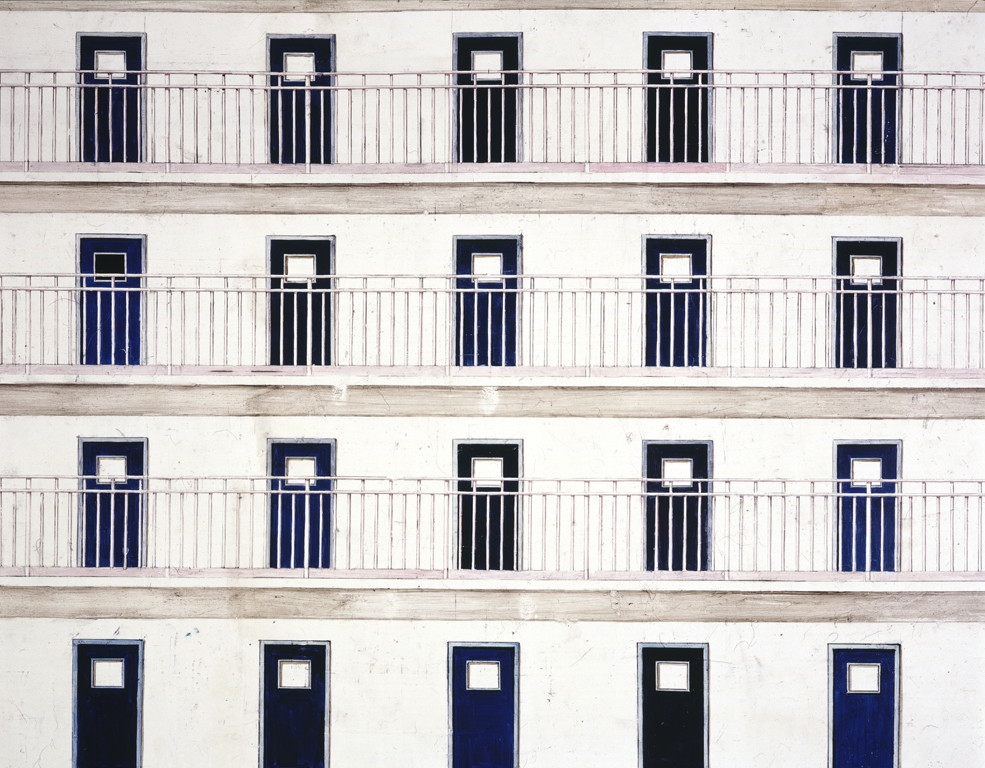
\includegraphics[scale=3.2]{doors.jpg}
    
    \vfill
    
    \large 
    \begin{tabular}{cc}
        Mitchell J. Abrams & Luke D. Gessler \\
        {\tt\normalsize mja284@georgetown.edu} & {\tt\normalsize lukegessler@gmail.com} \\
    \end{tabular}
    
    
    \vspace{0.3in}
    
    {\normalsize Georgetown University\\November 10, 2018}
    
\end{center}

\null\clearpage
\pagenumbering{roman}

\begin{quote}
    ``The acts of the mind, wherein it exerts its power over simple ideas, are chiefly these three: 1. Combining several simple ideas into one compound one, and thus all complex ideas are made. 2. The second is bringing two ideas, whether simple or complex, together, and setting them by one another so as to take a view of them at once, without uniting them into one, by which it gets all its ideas of relations. 3. The third is separating them from all other ideas that accompany them in their real existence: this is called abstraction, and thus all its general ideas are made.''
    
    -- John Locke
\end{quote}

\clearpage
\tableofcontents
\pagebreak

\pagenumbering{arabic}

\section{Introduction}

In this booklet, we aim to acquaint you with the most fundamental concepts needed to use Python for linguistic analysis. We hope that after completing this booklet you will be empowered to independently find the tools you'll need to solve problems you might have in analyzing your own linguistic data.

\subsection{Natural languages and programming languages}

As a linguist, you know that natural languages are rife with ambiguity. This is not the case with programming languages: there are no cases like ``I shot an elephant in my pajamas''. For a given ``utterance'' in a programming language, there is \emph{exactly one} ``meaning'' that can be assigned to it\footnote{This is only true, though, for a given compiler/interpreter. Two different implementations may make different decisions about how to interpret certain constructs.}. 

This characteristic of programming languages is a source of bliss and agony. On the one hand, the computer will always do exactly what it tells you to. On the other hand, you may not always fully understand how the computer will interpret a certain construction, and a subtle mistake or misapprehension may lead to a subtle misbehavior on the computer's part. (But as far as the computer is concerned, of course, it is behaving correctly.)

It is a fact of programming that there will often be times when you will grow frustrated at the computer's lack of ``common sense'', as it mechanically and literally interprets your programs and refuses to accommodate you by repairing and inferring information, as a human interlocutor would. But keep in mind that this rigidity can also be a source of bliss---once you have a complete knowledge of the computer's behavior, you will be assured that your program will behave as expected.


\subsection{Python at a glance}
Python was invented in 1991 by a Dutch programmer named Guido van Rossum. Van Rossum aimed to make a computer programming language as understandable as plain English that was still just as powerful as other programming languages. 

Computer scientists and software engineers prize Python especially for how quickly it lets them prototype new software. Scientists, on the other hand, are particularly drawn to Python's huge library of ready-to-go software packages, which allow them to reuse code other people have written for getting common tasks done, e.g. statistical analyses, accessing Twitter, or extracting data from special file formats like Excel spreadsheets.

\clearpage
\subsection{Python 2 vs. Python 3}
At this time, there are two versions of Python that are used that are incompatible with each other. In this book, we will be using Python 3. You should be aware, however, that Python 2 exists and that it behaves in slightly different ways. The two most important differences are that in Python 2 the \pyi{print} statement does not require parentheses, and the division operator only returns whole numbers:

\begin{python}
# Python 2
print 3/2
=> 1
# Python 3
print(3/2)
=> 1.5
\end{python}



\section{Hello, world}

Just like the Spotify app or a Google Chrome, Python is a piece of software that needs to be installed before it can be run. We recommend that you get started using an online service as described in \ref{sec:replit} and then eventually work on installing Python on your own machine as described in \ref{install}.

\subsection{Running Python with Repl.it}
\label{sec:replit}

\begin{figure}[ht]
    \centering
    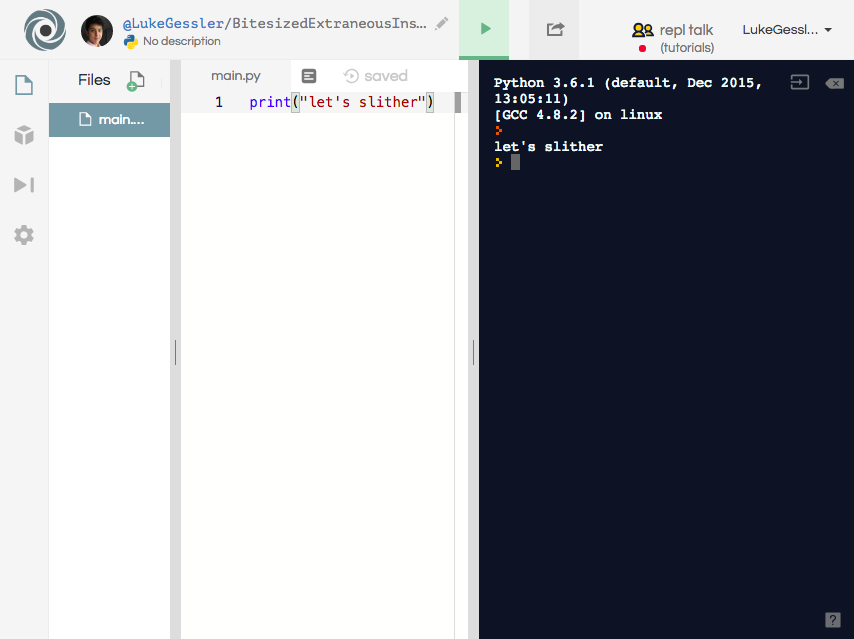
\includegraphics[scale=0.33]{replit_2.png}
    \caption{A successful ``hello, world'' in Repl.it}
    \label{fig:replit2}
\end{figure}

Repl.it is a web app that lets you write and execute Python code from your web browser. Let's set up an account and write a simple Python program to make sure everything works.

First, go to \url{https://repl.it} and create an account. After you're finished with registration, you should see a red ``+'' button in the bottom right corner of your screen. Hover over it, and click the sub-button that says ``Python3 repl'', as seen below:

\begin{center}
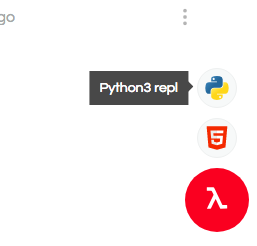
\includegraphics[scale=0.5]{replit_1.png}
\end{center}

Now you will see a white screen that has a text editor, as well as a black screen next to it. In the text editor, type \pyi{print("let's slither")} and hit the {\tt run} button at the top of the page. If everything's gone well, you should see {\tt let's slither} appear in the black screen to the right after you run your program, as in figure \ref{fig:replit2}.

What just happened? In short, Python read the text we gave it, determined that its meaning was `print {\tt let's slither}', and acted upon the meaning it recognized by displaying {\tt let's slither} in the black screen. If that seems vague, don't worry---we'll get more into the details of this in \ref{sec:repl}.

Congratulations, you're ready to start writing some Python!

\subsection{{\slshape Advanced}: Installing Python on your machine}
\label{install}

Installing and maintaining Python on your machine can take some elbow grease. We don't recommend that you do it right away. 

When you're ready to start working on bigger projects, however, you'll need to get an installation on your machine. The easiest way to do this is by installing Anaconda\footnote{\url{https://www.anaconda.com/download/}}. You can think of Anaconda as a batteries-included version of Python that has all the extra software for scientific computing that you otherwise would have had to track down and install yourself.

\section{Basic Python}

Now that you have a Python environment set up, we can begin learning the elements of Python's grammar.

\subsection{Python's ins and outs}
\label{sec:repl}

Let's take a step back for a moment. As you saw in section \ref{sec:replit}, when you provide Python with an \textbf{input} (the text you typed in the box), it \textbf{interprets} your input, and then it produces some \textbf{output}. In \ref{sec:replit}, you gave Python your input by typing it into the text editor and then hitting \emph{run}. 

Another way of giving Python your input is by using the \textbf{REPL}. REPL stands for read-evaluate-print loop\footnote{This window is also commonly called a ``console'' or ``terminal''. In the context of Python, you may treat these terms as equivalents of REPL.}. In Repl.it, you can find the REPL in the black window to the right of the text editor. 

Let's try something simple: click in the window, and type \pyi{2 + 2}. Python will take this \textbf{input}, \textbf{interpret} it, and display its \textbf{value}. As it turns out, the value of \pyi{2 + 2} is \pyi{4}, and Python should agree: 

\begin{center}
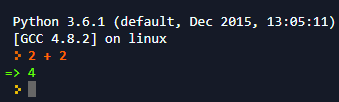
\includegraphics[scale=0.7]{2plus2.png}
\end{center}

When an entire file full of Python code is interpreted, its interpretation proceeds in more or less the same way as if every line had been typed into the REPL. However, the REPL has the advantage of giving you immediate feedback. You will see that this is useful as we proceed and start having to grapple with types of data that aren't as familiar as numbers.

There is one difference about the REPL worth noting: in a Python program, nothing is displayed in the output unless it appears inside \pyi{print}. In the REPL, the value of every line is repeated back you. (It's in the name: ``print''!)

\begin{exercises}
\item What should happen if you type \pyi{2 + 2} into the {\bf text editor} (not the REPL) and hit run? Is this the same as what would happen if you typed \pyi{print(2 + 2)} instead? Try doing both to see if you are correct. \\
\end{exercises}


\subsection{Numbers}
\label{sec:expressions}

In section \ref{sec:repl}, you saw how a simple input like \pyi{2 + 2} can be interpreted into an output, \pyi{4}. Inputs like \pyi{2 + 2} are called \textbf{expressions}. Number expressions behave mostly as you'd expect them to. We can add and subtract\ldots

\begin{python}
2
=> 2
2 + 2 
=> 4
2 - 1 + 3
=> 4
\end{python}

\noindent \ldots as well as multiply and divide:

\begin{python}
2 * 1 + 3
=> 5
2 * (1 + 3)
=> 8
3 / 4
=> 0.75
\end{python}

\noindent We refer to the mathematical symbols like \pyi{+} and \pyi{/} as \textbf{operators}. Of course, there are many other kinds of expressions in Python, but let's begin with these.

\begin{exercises}
\item The exponent operator in Python is \pyi{**}. \pyi{3 ** 2} is \pyi{9} ($3^2$), and \pyi{49 ** (1/2)} is \pyi{7} ($\sqrt{49}$). Use an expression to find the sum of the numbers 1 through 3 squared, i.e. $1^2 + 2^2 + 3^2$.
\item Sam Sociolinguist is analyzing her corpus of speech recorded in the graduate student lounge. 

She observed that Cam Computational uttered 3 sentences that contained the phrase ``it is the case'', which contained {\tt 3, 2, 4} clauses respectively, and that Cam's other 5 sentences were {\tt 4, 1, 1, 2, 1} clauses long, respectively. 

On average, how many clauses did Cam's ``it is the case'' sentences contain? What about all of them together?

\item Use an expression to find the average amount of money you've spent per day on transportation over the last few days.
\item \hard Write an expression that evaluates to \pyi{24} using only the numbers {\tt 5, 7, 5, 6}. 
\item \harder Use the numbers {\tt 1, 9, 9, 6} in exactly that order to compute the following numbers: {\tt 28, 32, 35, 38, 72, 73, 76, 77, 100, 1000}. You may insert parentheses and use any of the operators we have discussed so far.
\end{exercises}

\subsection{Functions}
\label{sec:functions}

In the exercises in section \ref{sec:expressions}, there were \emph{meaningful quantities} that we were interested in (like our average transportation expenses). What if we wanted to repeatedly find a meaningful quantity like this, like the result of adding two numbers and then dividing them by two? 

So far, the only way we have to do this is to manually type e.g. \pyi{(3 + 2)/2}, or \pyi{(7 + 10)/2}, every time we want to know the quantity for some new pair of numbers. Intuitively, we recognize that this seems like more work than we should be doing, because in these two expressions there is some kind of process that's common to them. (That is, adding two numbers and then dividing them by two.)

Python, like most other programming languages, has \textbf{functions} that allow us to associate a \textbf{name} with a \textbf{procedure}. The procedure is just a series of commands that tells it how to compute an output based on some kind of input. An easy example is a function that finds the area of a rectangle:

\begin{python}
def rect_area(width, height):
    return width * height

4 * 6
=> 4
rect_area(4, 6)
=> 24
\end{python}

Let's go through this function definition bit by bit. The \pyi{def} is a special, fixed keyword that tells Python we are defining a function. Next comes the name of the function, which we get to choose. In this case, we chose to call it \pyi{rect_area}, but it could have been something else as well, like \pyi{area} or \pyi{rectangle_area}. 

Next come the \textbf{arguments} of the function, which are names that stand in for the inputs we will give our function later when we actually know what they are. The colon tells Python that we're ready to begin describing how our function gets its output, and we begin the next line with four spaces. The \pyi{return} tells Python that we want to supply the result of the following expression as the output of this function.

Note that the body of the function is indented. Python needs this space in order to tell where the function ends. You may use either tabs or spaces to create this space, as long as you are consistent. The Python community tends to prefer using four spaces.

After the function has been \textbf{defined}, we can \textbf{call}\footnote{There are many synonyms programmers use for the act of calling a function: other common ones include \emph{invoke}, \emph{dispatch}, and \emph{evaluate}.} it to find its output given some inputs. As we can see for our example, the syntax for this is just the name of the function followed by its arguments, separated by commas.

Try typing the \pyi{rect_area} function into your Repl.it text editor, and hit ``run''. Your function has been loaded into the REPL! You should be able to type \pyi{rect_area(5, 5)} in the REPL and see the value \pyi{25} returned. 

In general, we recommend that you follow this three-step cyclic workflow: (1) write functions in the text editor, (2) hit ``run'' to load the REPL with your functions, (3) try calling your functions, examine the output, and think about what changes might need to be made.

\begin{exercises}
  \item Write a function called \pyi{cube} that computes the cube of a number. 
  \item Write a function that computes the perimeter of a rectangle, $2\times w + 2\times h$.
  \item Write a function that takes a single argument \pyi{x} and produces the output $x^2 + (x+1)^2 + (x+2)^2$.
  \item \label{exer:pythag} Write one function \pyi{square(x)} that computes the square of a number, and another function \pyi{square_root(x)} that computes the square root of a number. Write a function in terms of these functions that finds the longest edge of a right triangle, i.e. $c = \sqrt{a^2 + b^2}$.
  \item \label{exer:quadratic} \hard The quadratic formula, which you learned in high school algebra, is $x = \frac{-b \pm \sqrt{b^2-4ac}}{2a}$. Implement this as two Python functions: one for the value produced with a $+$, and one for the value produced with a $-$.
  
  \item \harder Complete exercise \ref{exer:quadratic}, except with one Python function instead of 2. Hint: add another argument to the function, \pyi{d}. If \pyi{d} is \pyi{1}, the function should produce the $+$ version of the value, and if \pyi{d} is \pyi{-1} , the function should produce the $-$ version of the value. E.g.:
  
  \begin{python}
  quadratic(1, 0, -1, 1) 
  => 1.0
  quadratic(1, 0, 1, -1)
  => -1.0
  \end{python}
  
  \item \hardest Suppose you have a function \pyi{f(x)} that takes a numeric x and returns some kind of numeric output. Other than that, you don't know anything about this function. Write a function \pyi{f_deriv(x)} that computes an approximation of the derivative of \pyi{f}, $\frac{f(x + 0.0001) - f(x)}{0.0001} \approx \lim_{h\rightarrow0} \frac{f(a+h)-f(a)}{h}$. If \pyi{f} changes, your \pyi{f_deriv} should not need to be changed in order to work properly.
\end{exercises}



\subsection{Variables}

Expressions will often become so big that they become too inconvenient to keep all on one line. Suppose that a phoneticist is conducting a study that involves measuring the average $F_0$ before and after a subject receives a stimulus, as well as the combined average. Pre-stimulus $F_0$'s were {\tt 179.66, 130.70, 166.19}, and post-stimulus $F_0$'s were {\tt 174.47, 135.78, 206.91}. We'd compute the averages like this:

\begin{python}
(179.66 + 130.70 + 166.19) / 3
=> 158.85
(174.47 + 135.78 + 206.91) / 3
=> 172.38666666666666
(((179.66 + 130.70 + 166.19) / 3) 
+ (174.47 + 135.78 + 206.91) / 3) / 2
=> 165.61833333333334
\end{python}

\noindent It's doable, but inconvenient and error-prone. 

\textbf{Variables} solve this problem by letting you store intermediate values for later use. Let's work that example again, this time using variables:

\begin{python}
pre_avg = (179.66 + 130.70 + 166.19) / 3
post_avg = (174.47 + 135.78 + 206.91) / 3
combined_avg = (pre_avg + post_avg) / 2
combined_avg
=> 165.61833333333334
\end{python}

\noindent Much less work! Note that this time the REPL didn't display the value of the expression back to us until we typed \pyi{total_avg} on its own. This is a convention the REPL follows: if a line of code \textbf{assigns} a \textbf{value} to a \textbf{variable}, it does not display anything.

Let's look a little more closely at the syntax of variable assignment in Python. Its form is \pyi{var = expr}. The \pyi{=} might make it seem that after \pyi{var} receives its value (the result of evaluating the \pyi{expr}), its value can never change. This is how equality works in mathematics: if we were in a high school math class and we read that $x = 2, y = x + 2$, we would conclude that $y$'s value must be $4$, and only $4$. 

This is not how \pyi{=} works in Python, however. Consider this Python code:

\begin{python}
x = 2
y = x + 2
y
=> 4
y = y + 3
y
=> 7
\end{python}

\noindent Even though on one line we said that \pyi{y = x + 2}, we later modified \pyi{y}, changing its value from 4 to 7! Python's \pyi{=} operator, while it looks like the mathematical $=$, actually means something quite different\footnote{It is unfortunate that Python uses \pyi{=} this way. It's worth noting that other programming languages express assignment differently: in the old-school AI language Lisp, the equivalent expression is {\tt (set! var expr)}, and in OCaml, it is {\tt var := expr}}.

So, mathematical equality is a misleading way to think about Python's \pyi{=}. A better way of thinking about \pyi{=} is to imagine that every variable corresponds to a box, and that the contents of that box can change, while the name that refers to that box stays the same.

\begin{exercises}
\item Variables can be defined inside of functions, as well. For example, we could have written our \pyi{square} function this way:

\begin{python}
def square(x):
    product = x * x
    return product
\end{python}

Write a function that computes the distance between two points, \\$\sqrt{(y_2-y_1)^2 + (x_2-x_1)^2}$, using variables to break the expression into smaller chunks. The head of your function should look like this: \pyi{def dist(x1, y1, x2, y2):}.

\item \label{exer:assign}\hardest Consider this code:
\begin{python}
y = 1
x = y
y = y + 2
\end{python}
\noindent What should the values of \pyi{x} and \pyi{y} be now? (Don't feel bad if you're not sure---it is not obvious.) Evaluate this code in the REPL. Are the values what you expected? Why do you think the values are what they are?
\end{exercises}

%Up until now, we've been working with values directly in the terminal, as in the case of doing mathematical operations with numbers. But what if you want to use numerical or string values later for another purpose? We can actually do this by storing our values in a reserved memory location, a \textbf{variable}. In other words, a variable holds our value. So we have a variable called "num" to represent 4. The process of creating a variable to hold a value is called \textbf{assignment}. This simple action becomes important later on when we want to keep track of values in our code and understand what our values represent. 

%Lets go through variable assignment and see how it can be useful. First, we will create a variable \textbf{first\_name} and \textit{assign} it a value \textbf{"wug"}. Here we are working with string values, and therefore need quotes surrounding the text. We will cover strings more in section 3.7. 


%\begin{center}
%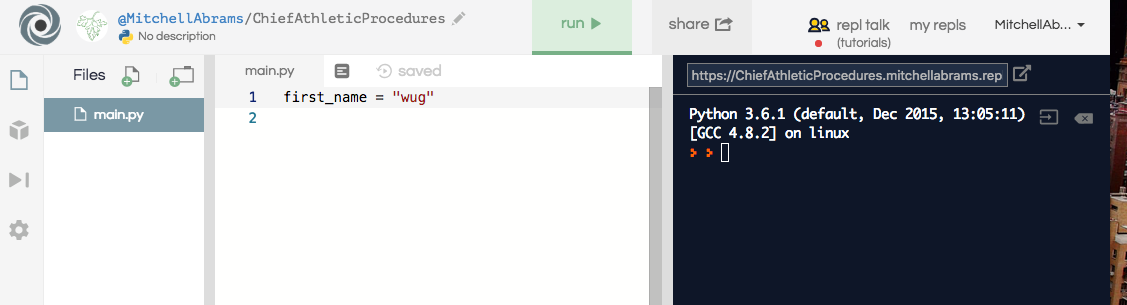
\includegraphics[scale=0.5]{replit_3.png}.png}
%\end{center}

%This \textit{assignment statement} contains a variable on the left and its assigned value on the right, assigned with the equal sign operator. Now our variable \texit{first\_name} holds our value for us. As you can see, if you run the program nothing happens. This is because the program just stored our value in memory, but if we type the variable alone and print it, it outputs our value.

%include example

%Now we will use our variable with other variables. 

%include bigger picture example


\subsection{Strings}

A \textbf{string} is a sequence of characters, like \pyi{"wug"} or \pyi{'hisssss'}. Obviously, as a linguist, you will be working with strings a lot. 

To write a string, you may use apostrophes or quotes, or triple quotes:

\begin{python}
"a string"
'here, apostrophes\'ll need a backslash before them'
"\"here\", he says, \"quotes need a backslash\""
"but apostrophes won't"
'''
"Un-backslashed apostrophes and quotes'll be just 
fine", she said, "and multiple lines, too."
'''
\end{python}



There are some character sequences that have special meanings within strings, and the two most important ones are \pyi{\\n}, for starting a new line, and \pyi{\\t}, for a tab:

\begin{python}
print('one\ttwo')
one     two
print('one\n\ntwo')
one

two
\end{python}

With numbers, there were only so many basic functions we could apply to them. With strings, there are many more. \pyi{+} and \pyi{*} can be used on strings, with intuitive meaning:

\begin{python}
first_name = "Richard"
second_name = "Simmons"
first_name + " " + second_name
=> 'Richard Simmons'
'longcat is l' + 'o' * 10 + 'ng'
=> 'longcat is loooooooooong'
\end{python}

Strings also have \textbf{methods}. Methods are functions that are closely associated with a certain type of data. We'll talk more about them later, but for now, you should just know that they're written in the syntax \pyi{t.f()} instead of in the syntax \pyi{f(t)}, like a normal function. For example, strings have a \pyi{replace} method that replaces every occurrence of some pattern inside the string with another string:

\begin{python}
s = "blockchains will change the world"
s = s.replace("blockchain", "giant spreadsheet")
s 
=> "giant spreadsheets will change the world"
\end{python}

\noindent If you're curious, you can find a full list of Python's string methods in the official documentation\footnote{\url{https://docs.python.org/3/library/stdtypes.html\#string-methods}}.

\begin{exercises}
\item Use the \pyi{replace} method to turn \pyi{"Warden Greely's Nordic garden"} into \pyi{"Warten Greely's Nordic garten"}.
\item Use \pyi{+} and \pyi{*} to produce \pyi{"Buffalo buffalo buffalo Buffalo buffalo"} using only the variables \pyi{B = "Buffalo"} and \pyi{b = "buffalo"}.
\end{exercises}


\subsection{Types and exceptions}
Python has other data \textbf{types} that are not numeric. These include strings (sequences of characters), Booleans (the special words \pyi{True} and \pyi{False}), and many others. We will discuss each more in turn. For now, you should just be aware that they exist. If you want to find out what the type of something is, you can simply use the built-in function \pyi{type}:

\begin{python}
a = 2
type(a)
=> <class 'int'>
type(3.4)
=> <class 'float'>
type(True)
=> <class 'bool'>
type('spam')
=> <class 'str'>
\end{python}

Sometimes it makes sense to combine two variables that have different types. As we've seen, \pyi{int} and \pyi{float}\footnote{\pyi{int} stands for integer, and you can think of \pyi{float} as a synonym for ``decimal number''. The two are distinguished in Python because computers can work with \pyi{int}s much more quickly than with \pyi{float}s.} can combine with each other without any difficulty:

\begin{python}
x = 13.2
y = 2
type(x)
=> <class 'float'>
type(y)
=> <class 'int'>
z = x / y
z
=> 6.6
type(z)
<class 'float'>
\end{python}

On the other hand, it doesn't always make sense to combine two values that have different types. What should the expression \pyi{1 + "spam"} evaluate to? In some sense, this expression is odd because we are trying to combine two types that aren't very similar: one is a number, and the other is a bunch of characters. Python chooses to disallow this operation, so it throws an \textbf{exception}:

\begin{python}
1 + 'spam'
Traceback (most recent call last):
  File "python", line 1, in <module>
TypeError: unsupported operand type(s) for +: 'int' 
           and 'str'
\end{python}

\noindent The \pyi{TypeError} is telling us that the \pyi{+} operator was given two values it didn't know how to add because of their types.

What if we really did want to make a number a part of a string, though? Python has built-in functions for cases like these that take a value and transform it into a sensible equivalent in the target type:

\begin{python}
pre_avg = (179.66 + 130.70 + 166.19) / 3
pre_avg
=> 158.85
str(pre_avg)
=> '158.85'
'Pre-stimulus average: ' + str(pre_avg)
=> 'Pre-stimulus average: 158.85'
\end{python}

These are the types we've seen so far. You can find a complete list in the official Python documentation\footnote{\url{https://docs.python.org/3/library/stdtypes.html}}.

\vspace{1em}\noindent \begin{tabular}{|c|c|c|c|}
\hline
\bf Name & \bf Description & \bf Examples & \bf Conv. Function \\\hline
integer & an integer & \pyi{0, -2, 3} & \pyi{int} \\\hline
float & a decimal number & \pyi{0.0011, 1.1e-3} & \pyi{float} \\\hline
string & a sequence of characters & \pyi{'word', "barn"} & \pyi{str} \\\hline
boolean & true or false & \pyi{True, False} & \pyi{bool}\\\hline
\end{tabular}\vspace{1em}

Let's make another version of our \pyi{square} function that prints its output instead of returning it. Type this into your text editor, and see what the output is when you run it:

\begin{python}
def square(x):
    return x * x

def square2(x):
    prod = x * x
    print(str(x) + "^2 is " + str(prod))

print(square(3))
square2(3)
\end{python}

\noindent Note that in \pyi{square2} we don't have to \pyi{print} its output, since it prints the result instead of returning it. Functions are allowed to end without a \pyi{return} in Python, in which case the function returns a special \pyi{None} value:

\begin{python}
print(square2(3))
3^2 is 9
None
\end{python}

% no exercises
\clearpage

\section{Working with language data}

Congratulations, you have now reached the point where you can begin working with real language data! There's still some Python left to learn, but you will master it as we go along.

\clearpage

\subsection{Getting started with Natural Language Toolkit} 

We will be using the \textbf{Natural Language Toolkit (NLTK)}\footnote{\url{https://www.nltk.org/}}. NLTK is a library of commonly used linguistic corpora and tools. To get started with NLTK, clear your Repl.it text editor and add this line:

\begin{python}
import nltk
\end{python}

\noindent The \pyi{import} keyword tells Python that we want to use a \textbf{package}. A package is just someone else's Python code that has been made publicly available. You will always need to make sure that the statement \pyi{import nltk} has been executed before you attempt to use anything in NLTK.

Now, hit \textbf{run}. In your REPL, type \pyi{nltk.download("gutenberg")}. This will download the full text of several books. Under the \textbf{Files} menu on the left side of your Repl.it screen, you should see a folder named \textbf{nltk\_data}. The texts have been stored under this folder.

Next, type \pyi{nltk.download("punkt")} in your REPL. This will download the Punkt tokenizer. You don't need to worry about what this does yet---we'll just need it under the hood for what we're about to do.

\begin{exercises}
\item Check out at the texts you just downloaded under the \textbf{nltk\_data} folder.
\item \hard Type \pyi{nltk.download()} in your REPL. Take a look at the other packages that are available for download. (Be careful if you're using Repl.it to do this---Repl.it workspaces have limited storage, and attempting to download a large NLTK package might cause problems.)
\end{exercises}

\subsection{Lists}

Let's find out what we got! We will now load all the sentences contained in Lewis Carroll's \emph{Alice's Adventures in Wonderland}. Then we will take one of them and inspect the words it contains:

\begin{python}
sents = nltk.corpus.gutenberg
                         .sents("carroll-alice.txt")
words = sents[7]
words
=> ['I', 'shall', 'be', 'late', "!'"]
type(words)
=> <class 'list'>
\end{python}

\noindent You are seeing Python's \textbf{list} data type. A list is simply a collection of values stored in a certain order. While the list is conceptually simple, you will see that it is very powerful.

Continuing from above, let's try retrieving individual items from the list: 

\begin{python}
words[0]
=> 'I'
words[1]
=> 'shall'
words[4]
=> "!'"
words[-1]
=> "!'"
words[0] + words[-1]
=> "Late!'"
\end{python}

\noindent We refer to the number inside of the square brackets as the \textbf{index}, which corresponds to a position within the list. Something that might surprise you is that we started counting at 0 instead of 1.\footnote{This is a convention followed in most programming languages. If it seems arbitrary and perhaps unnecessary, that's because it is. See the dedicated Wikipedia page: \url{https://en.wikipedia.org/wiki/Zero-based_numbering}} A consequence of this is that although there are 5 items in the list, attempting to access index 5 (\pyi{words[5]}) fails, because it actually refers to the non-existent 6th element:

\begin{python}
words[5]
Traceback (most recent call last):
  File "python", line 1, in <module>
IndexError: list index out of range
\end{python}

We can also get spans of words. These spans are called \textbf{slices}:

\begin{python}
words[0:5]
=> ['I', 'shall', 'be', 'late', "!'"]
words[0:2]
=> ['I', 'shall']
\end{python}

\noindent Slices have a start index and an end index. However, as you can see, the item in the left index is \emph{included}, while the item in the right index is \emph{excluded}. Why not include both? One reason for this is that defining slices this way lets you use the \pyi{len}, which tells you the length of a list, as a slice's right index:

\begin{figure}
    \centering
    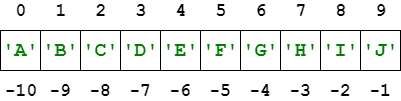
\includegraphics[scale=0.6]{list_indexes.png}
    \caption{Indexes for a list of length 10.}
\end{figure}

\begin{python}
len(words)
=> 5
words[1:len(words)]
=> ['shall', 'be', 'late', "!'"]
\end{python}

\noindent You can also omit one or both of the slice indexes, as well as use negative indexes:

\begin{python}
words[:2]
=> ['I', 'shall']
words[2:]
=> ['be', 'late', "!'"]
words[-2:]
=> ['late', "!'"]
\end{python}

It turns out that many other types in Python support the indexing and slicing operations, as well.\footnote{The object we loaded into the variable \pyi{sents} at the beginning of this lesson is one of them. While it is actually a more complex kind of structure, it still supports these operations, which is how we were able to pull the 8th sentence out of it using \pyi{words = sents[7]}.} Strings, for example, are among them:

\begin{python}
s = "I shall be late!'"
s[0]
=> 'I'
s[-6:]
=> "late!'"
\end{python}

There are two common ways of adding content to a list. You may either use \pyi{+} with another list, or you may use \pyi{list}'s \pyi{append} function:

\begin{python}
chars = ['Alice', 'Pat', 'Cheshire Cat']
chars.append('Mad Hatter')
chars
=> ['Alice', 'Pat', 'Cheshire Cat', 'Mad Hatter']
chars = chars + ['Queen of Hearts','King of Hearts']
chars
=> ['Alice', 'Pat', 'Cheshire Cat', 'Mad Hatter', 
                'Queen of Hearts', 'King of Hearts']
\end{python}

There are two common ways to delete items. You can use \pyi{append}'s counterpart \pyi{pop}, or add two slices:

\begin{python}
words.pop()
=> "!'"
words
=> ['I', 'shall', 'be', 'late']
words[2:] + words[0:2] + ['indeed']
=> ['be', 'late', 'I', 'shall', 'indeed']
\end{python}

\begin{exercises}
\item \label{exer:alicehurt} Using the list \pyi{a = ['Alice', 'was', 'not', 'a', 'bit', 'hurt']}, construct these lists: \begin{enumerate}
    \item \pyi{['not', 'a', 'bit', 'hurt']}
    \item \pyi{['Alice', 'was', 'hurt']}
    \item \pyi{['Alice', 'hurt', 'a', 'bit']}
    \item \pyi{['a', 'bit', 'hurt', 'Alice', 'not']}
\end{enumerate}

(Hint: remember that if you have a string \pyi{'s'} you can surround it with brackets \pyi{['s']} to turn it into a list with one element.) 
\item What should the output of \pyi{a[:]} (using \pyi{l} from exercise \ref{exer:alicehurt}) be?
\item Find at least three different ways to form the list \\\pyi{['Alice', 'was', 'a', 'bit', 'hurt']} using the list in exercise \ref{exer:alicehurt}.
\item Use only the functions \pyi{pop} and \pyi{append} to turn the list \\\pyi{['many', 'a', 'strange', 'tale']} into \pyi{['many', 'a', 'tale']}.
\item Strings have a function called \pyi{join} that inserts the string in between every item in a list of strings it is given. E.g., \pyi{" ".join(['riper', 'years'])} \pyi{=> 'riper years'}. Find some of the sentences at the beginning and the end of \emph{Alice in Wonderland} using the \pyi{sents} variable from the beginning of this chapter, and use the \pyi{join} function on those sentences so you can read them in your REPL. 
\item Use slicing to turn the string \pyi{s = 'the voice of the shepherd boy'} into \pyi{'the shepherd of the boy'}.
\item \hard Louis Riesener has a list \pyi{a = ['not', 'bad', 'at', 'all']} and is trying to use it to create the list \pyi{['not', 'at', 'all']}. He tries to do it using the expression \pyi{a[0] + a[-2:]}, but Python gives him an error: \pyi{TypeError: must be str, not list}. What is the problem with Louis's code? How would you fix it?
\item \harder Compare these two code segments:

\begin{python}
# segment 1
a = [1, 2]
b = a
a.append(3)
print(b)

# segment 2
a = [1, 2]
b = a.copy()  # or a[:]
a.append(3)
print(b)
\end{python}

What should the value of \pyi{b} be at the end of each segment? Test your hypothesis in the REPL. Referring back to exercise \ref{exer:assign}, compare the behavior of lists with the behavior of numbers:

\begin{python}
y = 1
x = y
y = y + 2
\end{python}
\end{exercises}



\subsection{When (not) to assign}

You might have noticed that when we're making changes to our data, sometimes we use assignment, and sometimes we don't:

\begin{python}
x = 2
x = x + 1   # x is now 3
y = [1, 2]
y.append(3) # y is now [1, 2, 3]
\end{python}

\noindent With \pyi{x}, we evaluate the expression \pyi{x + 1} and assign the result back into \pyi{x}. With \pyi{y}, we use \pyi{append} to add \pyi{3} to the list, but we do \emph{not} do anything with the result of the expression \pyi{y.append(3)}. 

So what's going on here? Let's see what happens when we use the opposite strategy with either data type:

\begin{python}
x = 2
x + 1
=> 3
print(x)
=> 2

y = [1, 2]
z = y.append(3)
print(z)
None
print(y)
=> [1, 2, 3]
\end{python}

\noindent In the first case, the results make sense: we computed the quantity \pyi{x + 1} $=$ \pyi{3}, but did not assign it to any variable. But the second case might be more surprising. Unlike the expression \pyi{x + 1}, \pyi{y.append(3)} evaluates to \pyi{None}, and instead, a change is made to the list called \pyi{y}. It turns out that lists \emph{are} allowed to have their contents change, whereas numbers are not. 

In this respect, when a data type behaves like a number, we say it is \textbf{immutable} (not changeable), and when it behaves like a list, we say it is \textbf{mutable} (changeable). You will always need to assign the value of an expression like \pyi{x + 1} to a variable, and you will usually \emph{not} want to reassign the value of an expression like \pyi{y.append(3)}.

This difference in behavior may seem arbitrary and confusing. For now, all you need to remember is that in Python, numbers and strings are immutable. For all other data types, you should assume that it is mutable.

\begin{exercises}
\item Using examples similar to the ones above, show that strings are immutable in Python.
\item The indexing syntax can also be used for assignment. For example:
\begin{python}
a = ['odi', 'et', 'amo']
a[1] = 'ac'
print(a)
=> ['odi', 'ac', 'amo']
\end{python}

\noindent Does this assignment by index also work with strings?
\end{exercises}

\subsection{Counting words}

With what you've learned so far, there's already quite a lot of linguistic analysis you can begin to do. Earlier, we saw the words and sentences in \emph{Alice}. Now, let's try loading the raw text that's inside the file, without processing it at all:

\begin{python}
import nltk
path="nltk_data/corpora/gutenberg/carroll-alice.txt"
text = open(path).read()
text
=> '[Alice\'s Adventures in Wonderland by Lewis 
Carroll 1865]\n\nCHAPTER I. Down the ...'
\end{python}

\noindent This is the full text of \emph{Alice} as a string. It would not be very easy to work with this string directly: it is littered with newline characters, and it's not easy to tell where each word begins and ends.

NLTK comes with a ready-to-go \textbf{tokenizer}, which will take this raw text and break it into units that more or less correspond to words:

\begin{python}
from nltk import word_tokenize
words = word_tokenize(text)
words
=> ['[', 'Alice', "'s", 'Adventures', 'in', 
'Wonderland', 'by', 'Lewis', 'Carroll', '1865', 
']', 'CHAPTER', 'I', '.', 'Down', 'the', ...]
\end{python}

\noindent This is still a pretty low-level representation of our text, but it's much easier to work with.

NLTK includes a tool called \pyi{FreqDist} that will count the occurrences of words. Let's import it and apply it to our tokens:

\begin{python}
from nltk.probability import FreqDist
freqs = FreqDist(words)
\end{python}

\noindent \pyi{FreqDist} is a special kind of function that returns an \textbf{object} that has special \textbf{methods} that will help us investigate the word distribution\footnote{In Python terminology, it is specifically an \textbf{instance} of a \textbf{class}. Classes are like lists in that they can contain a lot of data and have special methods that they know how to do, but they are even more powerful.}. We can find the most common words in the text using FreqDist's \pyi{most_common} method. This method returns a list of every word used in the text sorted by frequency---let's just take a slice of the top 10 so we don't overwhelm ourselves:

\begin{python}
freqs.most_common()[:10]
=> [(',', 2418), ('the', 1516), ("'", 1127), 
('.', 975), ('and', 757), ('to', 717), 
('a', 612), ('it', 512), ('she', 506), ('of', 496)]
\end{python}

Not surprisingly, \emph{the} and \emph{of} made the top 10. But what is perhaps disappointing is that so many punctuation marks made it into the top 10. 

How could we get this punctuation out of our token list? First, let's note that strings have a method \pyi{isalpha} that returns \pyi{True} if a string only contains alphabetical characters, and \pyi{False} otherwise. If we could somehow use this as a criterion for whether or not we should include a token in our list, we'd have our answer\footnote{Actually, we only have an approximation. Some tokens like \emph{n't} or \emph{'s} are not entirely ``alphabetical'' (in the special sense \pyi{isalpha} assumes) because they contain an apostrophe.}.

Python's \textbf{list comprehension}\footnote{List comprehensions are directly inspired by set builder notation used in mathematics: $\{x^2\ |\ x \in \mathbb{N}_0 \wedge x \leq 5 \} = \{0, 1, 4, 9, 16, 25\} \approx$ \pyi{[x ** 2 for x in range(6)]}} will help us get this done with ease:

\begin{python}
filtered_words = [w for w in words if w.isalpha()]
filtered_words[:11]
=> ['Alice', 'Adventures', 'in', 'Wonderland', 'by', 
'Lewis', 'Carroll', 'CHAPTER', 'I', 'Down', 'the']
\end{python}

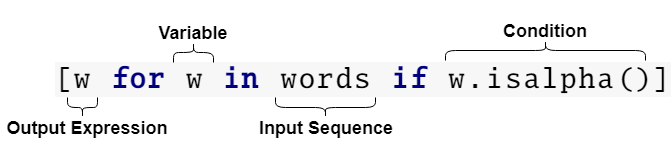
\includegraphics[scale=0.4]{listcomp.png}

\noindent There are four parts of a list comprehension. Let's walk through them for our case. The \textbf{input sequence} was a list with many strings inside of it. Every string in the list was bound, one by one, to the \textbf{variable} w. If the string's \pyi{isalpha} method returned true, then the list comprehension's \textbf{condition} was satisfied, and the \textbf{output expression} was evaluated and included in the new list\footnote{The output expression for this example turned out to be just \pyi{w} again, but it could have been anything in principle: for instance, we could have made it \pyi{w.lower()} to get the lowercase versions of the words, or something entirely unrelated, like \pyi{1}, for a list of \pyi{1}'s.}. If a word did not pass the \pyi{isalpha} test, it was discarded and not included in the new list.

Let's find a new \pyi{FreqDist} using this filtered list:

\begin{python}
filtered_freqs = FreqDist(filtered_words)
filtered_freqs.most_common()[:10]
[('the', 1516), ('and', 757), ('to', 717), 
('a', 612), ('it', 512), ('she', 506), ('of', 496), 
('said', 456), ('Alice', 394), ('I', 364)]
\end{python}

\noindent That looks a lot better! 

Note what the list elements look like: instead of strings, they are now \textbf{tuples}. Tuples will be useful whenever you want to associate pieces of information that are intimately related, such as a word with its lemma and part of speech: \pyi{('dogs', 'NNS', 'dog')}. A tuple is like a list, but it is immutable (cannot be changed):

\begin{python}
top10 = filtered_freqs.most_common()[:10]
top_word_tuple = top10[0]  
top_word_tuple
=> ('the', 1516)
top_word_tuple[0]
=> 'the'
top_word_tuple[1]
=> 1516
top_word_tuple[1] = 1513
Traceback (most recent call last):
  File "python", line 1, in <module>
TypeError: 'tuple' object does not support item 
                                          assignment
top_word, top_word_freq = top10[0]
top_word
=> 'the'
top_word_freq
=> 1516
\end{python}

\noindent Note how we assigned values to \pyi{top_word} and \pyi{top_word_freq}. If you know how many items a tuple (or a list, for that matter) contains, you can use this special syntax to assign their constituent values into their own variables. 
 
Let's try another list comprehension that will find every word with a frequency between 20 and 50:

\begin{python}
words_and_freqs = filtered_freqs.most_common()
med_freq_words = [t
                  for t in words_and_freqs 
                  if t[1] >= 20 and t1 <= 50]
# or
med_freq_words = [(word, freq)
                  for word, freq in words_and_freqs 
                  if freq >= 20 and freq <= 50]
# or
med_freq_words = [(word, freq)
                  for word, freq in words_and_freqs 
                  if 20 <= freq <= 50]
\end{python}

\noindent You should be able to figure out what's going on with our condition: the \pyi{<=} and \pyi{>=} operators mean just what you think they do, and we use the operator \pyi{and} to ensure that both of these are true. (Or we can chain the comparison operators, as in the last example.) 

These are the boolean operators you should be aware of:

\begin{center}
\begin{tabular}{|c|c|c|}
     \hline
     Operator & Example & Description\\\hline
     \pyi{>=, >, <=, <} & \pyi{1 > 2} $\rightarrow$ \pyi{False} & Numerical comparison \\\hline
     \pyi{==} & \pyi{[2, 1] == [2, 1]} $\rightarrow$ \pyi{True} & Equality test \\\hline 
     \pyi{\!=} & \pyi{'S' \!= 's'} $\rightarrow$ \pyi{True} & Non-equality test \\\hline 
     \pyi{and} & \makecell{\pyi{'a'.isalpha() and} \\ \pyi{len('a') == 1}} $\rightarrow$ \pyi{True} & Logical and  \\\hline 
     \pyi{or} & \makecell{\pyi{'abc'[1] \!= 'b' or} \\ \pyi{'c' in 'abc'}} $\rightarrow$ \pyi{True} & Logical or \\\hline 
     \pyi{not} & \pyi{not (len('a') == 1)} $\rightarrow$ \pyi{True} & Negation \\\hline 
     \pyi{in} & \makecell{\pyi{4 in (1, 2, 3)} $\rightarrow$ \pyi{False} \\ \pyi{'team' not in 'i'} $\rightarrow$ \pyi{True}}  & Non-equality test \\\hline 
\end{tabular}
\end{center}

\noindent Note that if you need to have a certain order of evaluation to be true, you should enforce it with parentheses:

\begin{python}
line = ['multitudinous', 'seas', 'incarnadine', '.']
print(not ',' in line or '.' in line)
=> True   # wrong--we don't want , or . in the line
print(not (',' in line or '.' in line))
=> False  # correct, since '.' appears in the list
\end{python}

Putting everything together, you should begin the exercises with this code as a starting point:

\begin{python}
import nltk
import nltk.probability
from nltk import word_tokenize
from nltk.probability import FreqDist

path="nltk_data/corpora/gutenberg/carroll-alice.txt"
text = open(path).read()
words = word_tokenize(text)
freqs = FreqDist(words)
filtered_words = [w for w in words if w.isalpha()]
filtered_freqs = FreqDist(filtered_words)
words_and_freqs = filtered_freqs.most_common()
\end{python}

\begin{exercises}
\item A problem with our \pyi{filtered_freqs} distribution is that words with different capitalizations were not combined. For instance, \pyi{'The'} was counted separately from \pyi{'the'}. Revise the list comprehension that produces \pyi{filtered_words} so that it also makes every word in the new list lowercase.
\item Write a list comprehension that finds all the word-frequency pairs for words that are longer than ten characters.
\item Strings have a function called \pyi{endswith} that returns \pyi{True} if the string ends with a certain string. E.g., \pyi{'ping'.endswith('ing')} $\rightarrow$ \pyi{True}. Write a list comprehension that finds all the words that end with \pyi{'tion'}.
\item Louis Riesener was unhappy with how \pyi{filtered_words} incorrectly excluded words like \emph{n't} and \emph{'s}, and wants to fix the list comprehension. So far, this is what he's written:

\begin{python}
punctuation = ['"', '\'', '.', '!', '?']
filtered_words = 
          [w for w in words if w != punctuation]
\end{python}

What is the problem with Louis' code? How would you fix it?
\item \label{exer:hapax} \pyi{FreqDist} has an interesting function called \pyi{hapaxes}. It returns a list of \emph{hapax legomena}, words that only occurred once in the text. Use a list comprehension to take the output of \pyi{most_common()} and filter it down into the list of hapax legomena. Compare your results with what is returned by \pyi{hapaxes()} to verify that you are correct. (Using the \pyi{==} operator to compare them should return \pyi{True}.) 
\item Write a function \pyi{only_x(words_and_freqs, x)} that returns a list like the one you constructed in exercise \ref{exer:hapax}, except filtered by words that appeared \pyi{x} times instead of only \pyi{1} time. 
\item \hard Use a list comprehension to find the total number of words in \emph{Alice} that end in \pyi('ing'). \emph{Hint:} Python has a \pyi{sum} function which returns the sum of a list of numbers, e.g. \pyi{sum([4, 5, 6])} $\rightarrow$ \pyi{15}.
\item \harder Write a list comprehension that finds all the word-frequency pairs for words that are longer than ten characters or begin with a capital letter that is followed only by lowercase letters. (Use string's \pyi{isupper} function.)
\end{exercises}

\subsection{Part of speech tagging}

With NLTK, getting a working part of speech tagger is as easy as two lines of code:

\begin{python}
nltk.download('averaged_perceptron_tagger')
from nltk import pos_tag
pos_tag(['all', 'these', 'letters', 'are', 
'pronounced', 'with', 'an', 'expulsion', 
'of', 'breath'])
=> [('all', 'PDT'), ('these', 'DT'), 
('letters', 'NNS'), ('are', 'VBP'), 
('pronounced', 'VBN'), ('with', 'IN'), 
('an', 'DT'), ('expulsion', 'NN'), 
('of', 'IN'), ('breath', 'NN')]
\end{python}

\noindent These tags\footnote{These tags are extended Penn Treebank tags. For a listing of these tags and their meanings, see \url{https://www.ling.upenn.edu/courses/Fall_2003/ling001/penn_treebank_pos.html}} will give us enough information for us to discern some basic linguistic structures. Let's tag \emph{Alice}:

\begin{python}
import nltk
from nltk import word_tokenize, pos_tag

path='nltk_data/corpora/gutenberg/carroll-alice.txt'
text = open(path).read()
words = word_tokenize(text)
tagged_words = pos_tag(words)
tagged_words[20:30]
=> [('to', 'TO'), ('get', 'VB'), ('very', 'RB'), 
('tired', 'JJ'), ('of', 'IN'), ('sitting', 'VBG'), 
('by', 'IN'), ('her', 'PRP$'), ('sister', 'NN'), 
('on', 'IN')]
\end{python}

Now, suppose we wanted to find every instance of a preposition (IN) followed by a gerund (VBG). Conceptually, in order to do this, we need to look at every item in the list and check its neighbor to the right. A list comprehension won't easily allow us to do this, so we need to reach for a different kind of strategy.

We're going to use the list comprehension's cousin, the \textbf{for loop}:

\clearpage\begin{python}
num_words_with_neighbor = len(words) - 1
positions_to_check = range(num_words_with_neighbor)
for i in positions_to_check:
    word_1, pos_1 = tagged_words[i]
    word_2, pos_2 = tagged_words[i+1]
    if pos_1 == 'IN' and pos_2 == 'VBG':
        print(word_1 + " " + word_2)
=> of speaking
for catching
without knowing
...
\end{python}

\noindent Our first step is to construct a list of every index we need to check. It turns out that this needs to be the length of the list minus one, because the last word in the list does not have a word to the right of it. We use Python's \pyi{range} function to help us make this list: \pyi{range(n)} constructs a list\footnote{It is not exactly a \pyi{list} (try typing \pyi{type(range(5))}), but this detail will not matter for us.} that contains all the numbers from \pyi{0} to \pyi{n - 1}. E.g., \pyi{range(5)} produces the elements \pyi{[0, 1, 2, 3, 4]}.

Now that we have this list, we will use the for loop to visit each element once. This syntax should look familiar to you from the list comprehension. We write code indented, below the for loop, to tell Python what we want it to do with each element of the list. We take the part of speech and form of each word, and then if the first one's tag is IN and the second one's tag is VBG, we print their forms separated by a space. 

The \textbf{if statement} should look familiar to you from the list comprehension, but here, it is being used to control whether a \textbf{block} of code will be executed, instead of whether an item will be included in a list. Here, whenever the condition is not satisfied, the if statement's body is not evaluated.

If statements are powerful, and you'll often find \pyi{if} joined by \pyi{else} and \pyi{elif} (else if).  For instance:

\begin{python}
def is_freezing(degrees, celsius):
    if celsius and (degrees <= 0):
        return True
    elif not celsius and (degrees <= 32):
        return True
    else:
        return False
\end{python}

\noindent These cases are checked successively, and as soon as Python finds a condition that is true, it evaluates the corresponding body, and does \emph{not} evaluate the bodies of any of the other statements that might be in the chain. 

Suppose we were interested in finding the frequencies of all of these prepositions before gerunds. This is a relatively simple modification of our code from above, using Python's \textbf{dictionary} type:

\begin{python}
num_words_with_neighbor = len(words) - 1
positions_to_check = range(num_words_with_neighbor)
freqs = {}
for i in positions_to_check:
    word_1, pos_1 = tagged_words[i]
    word_2, pos_2 = tagged_words[i+1]
    if pos_1 == 'IN' and pos_2 == 'VBG':
        if word_1 not in freqs:
            freqs[word_1] = 1
        else:
            freqs[word_1] = freqs[word_1] + 1
freqs
=> {'of': 33, 'about': 2, 'for': 15, 'on': 8, 
'in': 11, 'with': 1, 'by': 5, 'without': 13, 
'from': 3,  'after': 6, 'while': 1, 'down': 1, 
'at': 1, 'like': 1}
\end{python}

\noindent A dictionary is simply a way of converting a \textbf{key} into a corresponding \textbf{value}. And both keys and values are mutable, making dictionaries handy for counting tasks like this. You can use the functions \pyi{keys} and \pyi{values} to get the keys and values of a dictionary, or \pyi{items} to get them as a list of 2-tuples:

\begin{python}
freqs.items()
=> dict_items([('of', 33), ('about', 2), 
('for', 15), ('on', 8), ('in', 11), ...])
\end{python}

\begin{exercises}
\item Think about another tag pattern to look for that you think is interesting and modify the code above to find the items you're interested in.
\item How would you change the if statement testing parts of speech if you were interested in \emph{all} verbal forms after prepositions, and not just gerunds? (Hint: in this tagset, all verbal forms begin use string's \pyi{startswith} method.)
\item Based on what you saw in the last example in this chapter, answer the following questions about dictionaries:

\begin{itemize}
    \item How do you test whether an element exists as a key in a dictionary?
    \item How do you access a value in a dictionary with a key?
    \item How do you assign a value to a key in a dictionary?
\end{itemize}
\item Try to think of some words that will result in a wrong part of speech tag from the \pyi{pos_tag} function.
\item What do you think should happen if you deleted the \pyi{if/else} statement in the code snippet that calculates frequencies, and just replaced it with \pyi{freqs[word_1] = freqs[word_1] + 1} instead?
\item \label{exer:adjpairs} \hard Organize the code that printed all occurrences of IN, VBG above into a function \pyi{print_adjacent_pairs(tagged_words, tag_1, tag_2)} that allows you to find sequences of any two tags.
\item \harder Just like how lists had list comprehensions, dictionaries also have dictionary comprehensions. Can you infer what the syntax for this might be? (Try finding the dictionary comprehension that maps a number in \pyi{range(2,11)} to its square.)
\item \hardest Generalize the function you wrote in exercise \ref{exer:adjpairs} so that instead of accepting two tags it accepts a list of tags and prints all sequences of those tags. (Hint: you can nest for-loops, and you can use the \pyi{break} keyword to abort a for-loop, i.e. prevent the innermost for-loop from doing any more work.)
\end{exercises}

% moved a lot to scratch.tex

\section{Authorship attribution and stylometry}
\begin{quote}
\textit{``You see, but you do not observe.''}

-- Sherlock Holmes
\end{quote}

Authorship attribution is a task that tries to infer the characteristics of an author of some linguistics data, whether it's a letter, social media post, email, text message, book, etc. This is assuming that no one uses language in exactly the same way- we all have a "linguistic fingerprint" if you will. Typical authorship attribution cases usually deal with a piece of language data from an unknown author and compared to a set of possible candidate authors. While it's rare to find a "smoking gun" that will distinctly pick out an author from an open set of candidates, which actually happened in the Unabomber case \footnote{In 1995, an anomalously published manifesto from the unknown Unabomber titled “Industrial Society and Its Future” contained the phrase, “You can’t eat your cake and have it too", which an odd use of the more common idiomatic phrase "you can't have your cake an eat it too." This was enough to hint that the manifesto could be attributed to Ted Kaczynski. This evidence coupled with a constellation of other linguistic features was enough to label him as the author of the manifesto}, most authorship attribution cases compare a unknown document against closed set of possible authors. 

Traditional authorship attribution, which is routinely used in forensic applications, relies on identifying highly distinctive linguistic features that point to an author from a suspect pool. These features might include distinctive syntactic structures, idiomatic phrases, or lexical choices. As you might imagine, this method requires the background knowledge of a linguist who is an expert on language and can use intuition as a tool. Recently, authorship attribution has developed more statistical and machine learning approaches to authorship, which is referred to as \textbf{stylometry}. While this method is perhaps less transparent than traditional methods, it still yields great results, especially for documents that contain a lot of language data. Essentially, linguistic features such as word length, function words, pronoun choices, and short sequences of words (n-grams) among others, are fed into an algorithm that assigns the most likely candidate. 
%@article{mosteller1964inference,
%  title={Inference and disputed authorship: %The Federalist},
%  author={Mosteller, Frederick and Wallace, %David},
% year={1964},
% publisher={Addison-Wesley}
%}
\subsection{Case Study: Federalist Papers}
\begin{center}
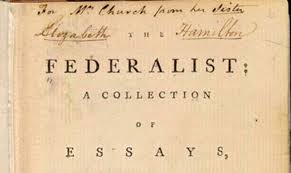
\includegraphics[scale=0.6]{federalist}
\end{center}

 A groundbreaking stylometry case study concerns the authorship of the disputed essays from the \textit{Federalist Papers}.  As a background, the Federalist Papers contained 85 essays that were written by John Jay, Alexander Hamilton, and James Madison between the years 1787 and 1788, and published under the pseudonym "Publius". While it is generally known which authors wrote which essays, there are still 12 that are claimed to be written by Madison and Hamilton.
 For this case, Mosteller and Wallace (1964) use statistical methods and Bayesian analysis to determine that the author of the disputed essays was actually James Madison. How did they do it? They approached their analysis by looking at \textit{function words} like prepositions, conjunctions, and articles. As function words carry little meaning, they are typically topic-independent and used more unconsciously, and therefore less susceptible to manipulation. Consequently, they turn out to be very robust features in determining authorship and are still used today in many modern methods and machine learning algorithms. 


\subsection{Case Study: A Cuckoo's Calling}
\begin{center}
    
\includegraphics[scale=0.6]{cuckoo}
\end{center}


A More recent case involves the authorship of the book titled \textit{The Cuckoo's Calling}. While this novel claims to be authored by Robert Galbraith, a reporter from \textit{The Sunday Times} suspected that the true author was JK Rowling, writing under a pen name. This question of authorship was taken to Dr. Patrick Juola\footnote{http://juolaassociates.com/}, the developer of JGAAP (Java Graphical Authorship Attribution Program), a program that does a  mathematical analysis of the degree of similarity across features- a system far more complex than the one used by Mosteller and Wallace. 

The system took many robust features into account, ones that only a computer program can efficiently count and compare. Some of the main features included the distribution and comparison of word length, common words, and 4-grams and bi-grams. 4-grams and bi-grams are known more generally as \textit{n-grams}, an \textit{n} sequence of characters or words that are very useful as authorship attribution features. Collecting and comparing all of the bi-grams (two adjacent words) like \textbf{"in the"} or \textbf{"after a"}, for example, can reveal distinctive language usage patterns. One author might use the tri-gram \textit{"it is a"} at a proportionally higher rate when compared to a corpus that represents a larger population or group. 

The method for this analysis involved Juola collecting known writings of Rowling and three other female novelists as comparison corpora. After comparing the novel to the styles of the four authors, the program matched the novel to writings of Rowling. While this form of analysis cannot prove that J.K. Rowling was the author, this stylometric approach shows that the writings styles of the novel and Rowling are very similar. 

Once J.K. Rowling was approached on this topic by \textit{The Sunday Times}, she admitted to writing the novel. While it certainly seems unnecessary that Rowling was approached on this question of authorship in the first place, considering that she wrote under a pen name for a reason, the case study shows how effective modern techniques and computer programs can be in determining authorship. It also highlights some of the linguistic features that are frequently compared and how difficult it would be for humans to keep track of them and notice patterns. One can imagine how time consuming it would be to count the character sequences in a text by hand. 

With these case studies in mind as a background on the field, we can use python as our tool to conduct our own authorship analysis. This time we'll look at the \textit{Bitcoin Papers}. 



\section{The Bitcoin whitepaper whodunnit}

On Halloween 2008, a paper titled \emph{Bitcoin: A Peer-to-Peer Electronic Cash System}\footnote{\url{https://bitcoin.org/bitcoin.pdf}} was posted to a cryptography mailing list\footnote{\url{http://www.metzdowd.com/pipermail/cryptography/2008-October/014810.html}} by a person calling himself Satoshi Nakamoto. The paper outlined a scheme for a kind of electronic currency that would rely on no governments or other central authorities, and would provide a measure of anonymity for its users. Two months later in January 2009, he released the first implementation of the software powering this currency. Today, there are about 17 million Bitcoins in circulation, valued at around \$10 billion USD.

Circumstantial evidence has led many to doubt Nakamoto's identity:

\begin{itemize}
    \item Nakamoto writes in English that, without fail, sounds native and is free of grammatical patterns characteristic of even an advanced L2 English speaker.
    \item None of Nakamoto's software was produced, commented, or documented using Japanese.
    \item Nakamoto has occasionally produced Britishisms such as ``bloody hard''.
    \item The first Bitcoins ever mined, which were mined by Nakamoto since he was the only user of Bitcoin at the time, were cryptographically signed with the text ``{\tt The Times 03/Jan/2009 Chancellor on brink of second bailout for banks}'', the title of an article that was written in the London newspaper \emph{The Times}.
\end{itemize}

\noindent This evidence, while obviously not enough to prove that Nakamoto's identity was false, was certainly enough to get people to think about who Nakamoto might be if he was not Nakamoto. Rumors of Nakamoto's true identity circulated for years, though evidence was scarce for any of the people Nakamoto was supposed to be.

In 2013, a blogger made the case that Nakamoto was in fact an American named Nick Szabo\footnote{https://likeinamirror.wordpress.com/2013/12/01/satoshi-nakamoto-is-probably-nick-szabo/}. To make his case, the blogger noted Szabo's lifelong interest in cryptocurrencies, Szabo's public description of a hypothetical system called ``bit gold'' published only a bit before the Bitcoin whitepaper, and a few other pieces of evidence. 

So far, all of this evidence was similar at least in kind to what others had brought to bear in making the case that they had found Nakamoto's true identity. But what was new in this allegation was the stylometric evidence given which the blogger claims are proof of Szabo's authorship of the whitepaper (quoted from the post):

\begin{itemize}
    \item Repeated use of ``of course'' without isolating commas, contrary to convention (``the problem of course is'')
    \item Expression ``can be characterized'', frequent in Nick’s blog (found in 1\% of crypto papers)
    \item Use of ``for our purposes'' when describing hypotheses (found in 1.5\% of crypto papers)
    \item Starting sentences with ``It should be noted'' (found in 5.25\% of crypto papers)
    \item Use of ``preclude'' (found in 1.5\% of crypto papers)
    \item Expression ``a level of'' + noun  (``achieves a level of privacy by…'') as a standalone qualifier
    \item Repeated use of [the] expression ``trusted third party''
    \item Expressions ``cryptographic proof'' and ``digital signatures''
\end{itemize}

\noindent Regardless of whether it should have been, this blogger's stylometric evidence was persuasive, and many in the Bitcoin community today still believe that Szabo is Nakamoto.

Your task in this next exercise will be to try to replicate some of these stylometric results using the exercise template. We have prepared three text files for you: one with the text of the Bitcoin whitepaper, one with the papers written by Nick Szabo mentioned in the article, and one with several cryptography papers written around the same time as the Bitcoin paper.

\begin{exercises}
\item Open the exercise template\footnote{\url{https://repl.it/@LukeGessler/Bitcoin-White-Paper-Stylometric-Analysis}} and create a fork by hitting the ``fork'' button.
\item Write a function that will find the frequencies\footnote{The frequency of a word is equal to the number of times it appears in the list divided by the total length of the list.} of the phrase ``of the'' across these three texts. (This will serve as a sanity check, since ``of the'' is sure to occur in all of them.)
\item Generalize your function so that it will check for the occurrence of any sequence of \emph{n} words.
\item Use your function to check for the stylometric factors identified by the blogger, such as ``digital signatures'', ``trusted third party'', ``for our purposes'', etc. Are you able to get the same results? (Hint: you might not be.)
\item Skim the text file with Szabo's papers in it. Just reading through it, is there anything that strikes you as peculiar about his writing style? Conduct a stylometric test to see if this ends up being more common in his and Nakamoto's writings. Come up with a few others if you can, including one that makes use of part of speech tags.
\item \hard Read over the blogger's arguments again. Are you convinced by their argument that these stylometric numbers are statistically significant? 
\end{exercises}


\section{Conclusion}
We hope this booklet has helped you master the most fundamental concepts needed for programming in Python and that it has given you a taste of the powerful analytic tools Python has to offer you. 

We recommend that you take a look at the NLTK book\footnote{\url{https://www.nltk.org/book/}} to learn more about what NLTK has to offer you. The book is also structured so that it teaches you Python as it teaches you about the specific offerings of the library.

There is a wealth of other materials that will help you learn Python in general, and it would be a good idea for you to try a few different ones to see which of them most suits you. We are particularly fond of a set of materials called Composing Programs\footnote{\url{http://composingprograms.com/}}. To get started on finding Python learning materials, we recommend you look at these threads on Hacker News\footnote{\url{https://news.ycombinator.com/item?id=17177186}} and /r/Python\footnote{\url{https://www.reddit.com/r/Python/comments/6vn0h9/best_python_resources_for_python_beginners_in_2017/}}

\subsection*{Acknowledgements}

Thanks to Georgetown University Graduate Student Government for funding the November 10, 2018 workshop, and to the Graduate Linguistics Student Association for securing the funding and handling the organization of the workshop. 

This booklet has drawn inspiration (and sometimes content) from these excellent works:

\begin{enumerate}
    \item Dave Evans'  CS 1120 slides: \url{http://www.xplorecs.org/class1}
    \item Structure and Interpretation of Computer Programs: \\ \url{https://sarabander.github.io/sicp/html/index.xhtml}
    \item The NLTK book: \url{https://www.nltk.org/book/}
\end{enumerate}

Cover art: Untitled (doors) by Toba Khedoori, 1996.\footnote{https://curiator.com/art/toba-khedoori/2}

Back art: Untitled by Toba Khedoori, 2008.\footnote{https://curiator.com/art/toba-khedoori/1}

\clearpage
\pagenumbering{gobble}

\topskip0pt
\vspace*{\fill}
\begin{center}

\includegraphics[scale=0.65]{chair.png}
\end{center}
\vspace*{\fill}
%\section{External listing highlighting}

%\pythonexternal{demo.py}

%\section{Inline highlighting}

%Definition \pyi{class MyClass} means \dots

\end{document}